% !TeX program = xelatex
% !TeX encoding = UTF-8
\documentclass{MathorCupModeling}
\usepackage{mwe,color,float}
\usepackage[linesnumbered,ruled]{algorithm2e}
\everymath{\displaystyle}

\extrafloats{100}
\bianhao{MC2305806}
\tihao{D}
\timu{\textbf{题目}}
\keyword{关键词两个之间分号隔开}
\begin{document}
	\begin{abstract}
		这里是摘要部分
	\end{abstract}

	\pagestyle{empty}
	\tableofcontents
	\newpage
	\pagestyle{fancy}

	\setcounter{page}{1}
	\section{问题的提出}
	\subsection{问题背景}
	改革开放以来,我国民航业蓬勃发展,越来越多的乘客选择乘坐飞机出行,飞行安全的重要性不言而喻。截至2022年3月21日,即“3.21”空难发生前,我国民航安全飞行达1亿零59万飞行小时,为我国历史最好安全记录。严重的飞行安全事故不仅会使航空公司蒙受经济损失,还威胁着乘客的生命财产安全。为科学管理,降低飞行事故发生的几率,综合现有数据进行监测并预警风险,总结出具有针对性和系统性的方案提升从业人员素质显得尤为重要。在航空安全数据分析中快速存取记录器(Quick Access Recoder,QAR)发挥着重要作用。目前我国民航业主要研究两方面:
	\begin{itemize}
		\item 超限事件的研究,分析及应用;
		\item 非超限数据的统计分析及应用。
	\end{itemize}其中,对于前者的分析着眼于超出阈值的部分,然而超出阈值的部分不完全是人为因素,可能为环境或飞机本身存在一定问题,若基于非人为因素对机组严以要求显然是不合理的。QAR超限可为航空安全管理和飞行训练提供数据支撑,而少量的QAR超限显然不具有说服性,故挖掘QAR全航段数据,基于不同飞行机组,航线,机场及特殊飞行条件下的飞行记录,建立数学模型,并分析之,评估各指标风险系数,针对性开展安全培训,排除安全隐患,改进安全绩效。
	\subsection{问题要求}
	\begin{itemize}
		\item \textbf{问题一}:由于QAR数据并不能保证绝对正确性,故应进行数据预处理减少错误数据干扰。在此基础上对附件1进行可靠性研究,提取关键数据项并分析重要程度。
		\item \textbf{问题二}:飞行过程往往通过一系列飞行操纵如:横滚、俯仰等以保证安全。国内航司主要以超限监控飞行动态,虽然能够快速分辨飞机状态偏差,但无法在较短时间内知道原因。为解决此问题,请依据附件1合理量化描述飞行操纵。
		\item \textbf{问题三}:除人为,环境,飞机本身缺陷外等因素外,仍有一定因素会影响超限的发生。请依据附件2分情况讨论超限并研究其基本特征。
		\item \textbf{问题四}:飞机运行数据研究往往由两大类组成,一类由LOSA获取,另一类则遵从相关学者建议,开展飞行技术评估。请依据附件3,建立数学模型以合理分析评估飞行员飞行技术。
		\item \textbf{问题五}:在QAR实现陆空实时传输的情况下,以航司安全管理人员的身份建立实时自动化预警机制,预防可能的安全事故,并依据附件1给出仿真结果。
	\end{itemize}

	\section{问题的分析}
	\subsection{问题的整体分析}
	该问题是一个关于航空安全风险及飞行技术的数据分析、建立预警模型的问题。
	
	\textbf{从分析目的看},

	\textbf{从数据来源、特征看},
	
	\textbf{从模型的选择看},

	\textbf{从编程软件的选择看},本题为大数据分析类,需要进行大量的数据预处理、数据分析、数据可视化,并依据各设问建立预警自动化只能预警机制,因此我们选择Python Jupyter对问题进行求解,其交互式的编程范式及轻量化,方便且高效。
	
	\subsection{问题一的分析}
	问题一的核心目的有以下几点:{\heiti 其一},\textbf{对真实的QAR数据进行预处理,去伪存真};{\heiti 其二},\textbf{分析研究附件一数据质量的可靠性};{\heiti 其三},\textbf{提取一项飞行安全的关键性因素,并定性及定量分析}。对于已给的数据集,数据在真实性、完整度、指标标准等方面存在一定缺陷,这导致我们在原始数据上不可直接进行分析,因此需要对其进行相应的预处理。此外附件1为8次航班的由起飞到降落的全过程的QAR数据,数据体量大,因此我们需要由特殊到一般,建立普适性模型,高效分析多张数据表格;同时我们还发现,数据维度较高,为得到关键性因此,考虑累计方差解释、层次聚类分析及熵权法,确定重要度较高指标,并对筛选出的指标进行合理性分析。
	\subsection{问题二的分析}
	\subsection{问题三的分析}
	\subsection{问题四的分析}
	问题四的核心目的在于\textbf{基于飞行参数对飞行员的技术进行评估}。但是附件3与附件1同样在数据完整度、指标标准等方面存在一定缺陷,因此我们也需要对其进行一定的预处理;同时,我们还发现附件3维度更高,飞行参数较多,对于模型的效率有一定影响,因此我们沿用问题一的想法,以累计方差解释确定重要因素较高的指标的个数,再以随机森林及极端梯度提升算法综合分析出与飞行员飞行技术重要程度较高的因素。但我们还发现,附件3中,飞行员资质为“C”类的占比仅为整体的$0.844\,\%$,因此我们综合多方面考虑,选择将该两项数据单独分析,剩余数据视为多分类预测。最后以筛选出的重要指标为自变量,飞行员的“不同资质”,即不同技术级(除“C”类)别为因变量,建立XGboost多分类预测模型,从而建立出基于飞行参数的飞行技术评估方法。同时,为探讨模型效果,我们绘制出模型的{\heiti 分类混淆矩阵热力图}、{\heiti 分类报告}、{\heiti ROC/AUC	曲线}等对预测结果进行合理性分析。
	\subsection{问题五的分析}

	\section{模型的假设}
	\begin{itemize}
		\item \textbf{假设一}:
		\item \textbf{假设二}:
		\item \textbf{假设三}:
		\item \textbf{假设四}:
	\end{itemize}
	\section{符号说明},
	\begin{center}
		\begin{tabularx}{0.7\textwidth}{c@{\hspace{1pc}}|@{\hspace{2pc}}X}
			\Xhline{0.08em}
			符号 & \multicolumn{1}{c}{符号说明}\\
			\Xhline{0.05em}
			$\mu$ & 样本平均数 \\
			$\alpha$ & 系数 \\
			$\beta$ & \\
			$\omega$ & \\
			$\sigma$ & 标准差 \\
			\Xhline{0.08em}
		\end{tabularx}
	\end{center}

	\section{模型的建立与求解}
	对于本题,本文模型的建立与求解部分主要分为数据的准备,模型的建立、求解、结果分析。
	\begin{itemize}
		\item \textbf{数据的准备}:对于给定的数据集进行预处理,方便后续模型的建立,以及多次航班的规范分析。
		\item \textbf{模型的建立、求解、结果分析}:对于给定的数据集,本文依据其特点,建立合适的模型,研究并量化分析影响飞行安全的因素。此外还需要分析飞行阶段操纵杆的过程变化情况,分析安全性。同时,还需要依据飞行参数对驾驶员飞行技术进行预测,并解释预测的合理性。最后需要结合上述问题,建立自动化智能预警机制,预防可能的安全事故的发生,给出仿真结果。
	\end{itemize}
	\subsection{问题一模型的建立与求解}
	对于问题一,我们首先分析数据的特点,依据时间特征及对应的各参量进行合理性分析,对错误值进行剔除,提高数据的真实性,并以此分析数据的可靠性;之后我们依据刘柳\textcolor{blue}{\cite{Paper:刘柳}}、龙海江\textcolor{blue}{\cite{Paper:龙海江}}学者的研究结成果,采用层次聚类法对多维度指标进行聚类分析,同时在此基础上利用主成分分析累计方差解释,确定影响飞行安全的关键性指标,并利用熵权法对其重要性进行量化分析。此外注重定性及定量的分析研究,结果与现实情况相近,选取结果良好。
	\subsubsection{附件1数据预处理}
	通过对附件1的8个Excel表格依此分析,并结合快速存取记录器(Quick Access Recoder,QAR)数据的特点,我们发现以下几点可能的错误方面:
	\begin{itemize}
		\item \textbf{起始时刻不为飞机开始运行时刻}:通过对8张表8次航班的全航段记录数据的逐一分析,我们发现表格“201404091701”记录器开始记录的时刻为2014年4月9日14时23分51秒,而该航班实际运行时间应该为2014年4月9日17时01分50秒,因此我们认为该表格的起始时刻不应为前者,而应是飞机开始运行的时刻。因此我们将该表格的起始时刻校正,即删除14时23分51秒的数据,保留17时01分50秒之后的数据。而对于其余表格并未发现相同错误。
		\item \textbf{相邻数据存在时刻上的重复且后续指标不一致}:利用Python的pandas库,对8张表格统一分析,发现所有表格均存在该方面的问题,即存在某同一时刻的数据,但后续指标却不一致,这是明显的QAR数据记录错误,究其原因,可能是由于该时刻被QAR连续记录两次,但指标发生变化,但为了保证数据的在时刻上的连续性,我们以这些重复时刻数据首次出现的为标准,将其保留,而另一条数据选择剔除。
	\end{itemize}

	经过上述处理后,为了再次验证数据在时刻层面的连续性,即每行记录的数据均间隔为1秒,我们对所有航班进行时刻点计算,均与处理后的数据记录条数一致,从而也反映出保留下的数据的合理性。

	同时我们发现,附件1的8张表格,前三行均属于表头类型,且有部分字段重复,若将其直接利用pandas读取,可能会对后续处理产生一定影响,因此我们根据附件1的字段中文说明,将8张全航段表格数据表头进行处理,且保证所有表格表头一致,方便后续处理。

	此外,通过读取附件1数据,查看其空缺值情况,发现“起落架”\textcolor{blue}{\footnote{这里指标名称已由原数据的英文修改为中文指标。}}该列数据缺失值较多,这里我们以附件1中表格“201404101159”为例,其空缺值情况如\textcolor{blue}{\cref{fig:附件1航班8缺失值}}所示。















	\textbf{熵权法(Entropy Weight Method, EWM)}是一种指标客观影响程度的量化方法。当信息熵越大时,信息的无序程度越大,此时,信息价值越小,指标权重就越小\textcolor{blue}{\cite{pewm1}}。其计算步骤如下:
	\begin{itemize}
		\item \textbf{Step1},指标正向化。由于数据集构成的指标类别不一,部分指标可能数值越大越好,部分指标可能越小越好,而有的可能在某一点取值最优,为方便、高效评价,我们需要进行指标正向化处理\textcolor{blue}{\cite{pewm2}}。其处理方法如下
		\begin{itemize}
			\item {\heiti 越大越优指标}
			\begin{equation}
				x'_{ij}=x_{ij} \label{fmax}
			\end{equation}
			\item {\heiti 越小越优指标}
			\begin{equation}
				x'_{ij}=\mathrm{max}\left(x_{ij}\right)-x_{ij} \label{fmin}
			\end{equation}
			\item {\heiti 在$\beta$处取值最优指标}
			\begin{equation}
				x'_{ij}=1-\frac{\left|x_{ij}-\beta\right|}{\mathrm{max}\left(\left|x_{ij}-\beta\right|\right)} \label{fmid}
			\end{equation}
		\end{itemize}
		\item \textbf{Step2},数据标准化。由于数据集构成的指标数据数量级存在差异、量纲不一,为消除上述情况对结果的影响,我们需要将各指标进行标准化处理,这里我们使用Min-Max方法。处理方法计算公式如下
		\begin{equation}
			r_{ij}=\frac{x'_{ij}-\mathrm{min}\left(x'_{j}\right)}{\mathrm{max}\left(x'_{j}\right)-\mathrm{min}\left(x'_{j}\right)} \label{Min-Max}
		\end{equation}
		\item \textbf{Step3},计算信息熵。进行上述处理后可得到由特征数据构成的矩阵$R\left(r_{ij}\right)_{m\times n}$,对于某一项指标的数据$r_j$,其信息熵为
		\begin{equation}
			E_j=-\frac{1}{\ln m}\cdot\sum\limits_{i=1}^{m}p_{ij}\ln p_{ij} \label{fentropyj}
		\end{equation}
		其中
		\begin{equation}
			p_{ij}=\frac{r_{ij}}{\sum\limits_{i=1}^{m}r_{ij}} \label{fpij}
		\end{equation}
		观察到\textcolor{blue}{\eqref{fpij}}中分母不可为$0$,且\textcolor{blue}{\eqref{fentropyj}}对数真数部分不能为$0$,因此,我们在进行\textbf{Step2}时,标准化区间的最小值设为$0.002$,可避免计算时的不合定义。
		\item \textbf{Step4},计算指标权重。其计算公式如下
		\begin{equation}
			\omega_j=\frac{1-E_j}{\sum\limits_{j=1}^{n}\left(1-E_j\right)} \label{fwj}
		\end{equation}
	\end{itemize}



	这里是图片的演示,见\textcolor{blue}{\cref{fig:picturename1}}。
	\begin{figure}[H]
		\centerline{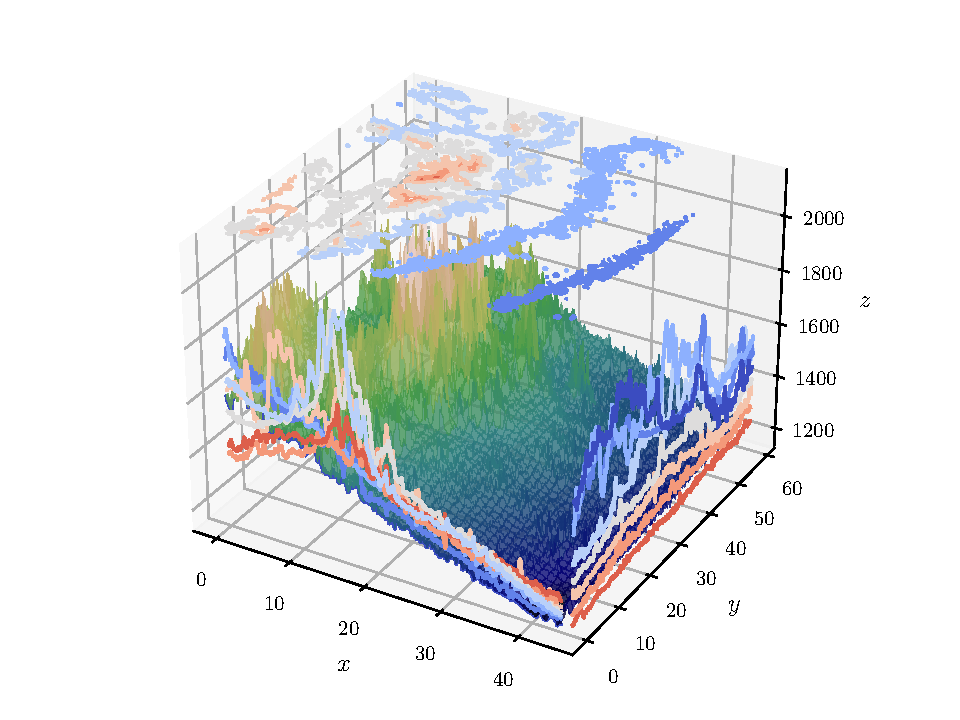
\includegraphics[scale=0.8]{三维网格图.pdf}}
		\caption{这里是图片的标题}\label{fig:picturename1}
	\end{figure}
	这里是第二张图片的延时,见\textcolor{blue}{\cref{fig:picturename2}}。
	\begin{figure}[H]
		\centerline{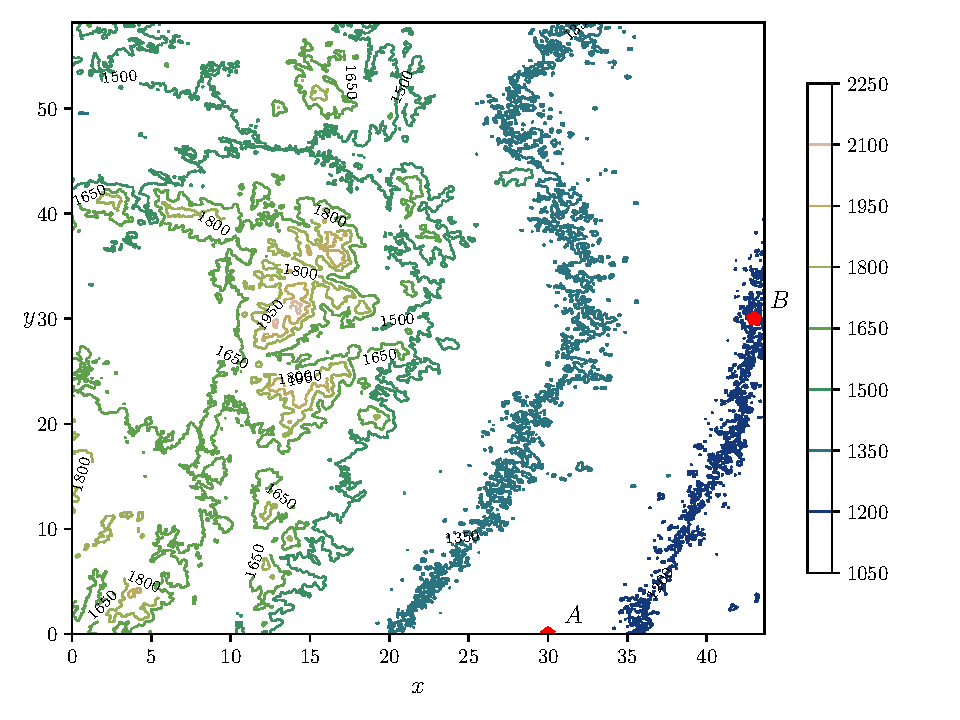
\includegraphics[scale=0.8]{等高线图.pdf}}
		\caption{这里是图片的标题}\label{fig:picturename2}
	\end{figure}
	假如这段话是引用了话,要有注释喔!\textcolor{blue}{\cite{p1}}
	这里我们还可以做个脚注。\textcolor{blue}{\footnote{脚注的内容}}

	这里我们做一个表格,三线表喔!见\textcolor{blue}{\cref{tab:tablename1}}。
	\begin{table}[htbp]
	\centering
	\caption{标题在这里!~}
	\setlength{\aboverulesep}{0pt}
	\setlength{\belowrulesep}{0pt}
	\scalebox{0.88}{
	  \begin{tabular}{ccc}
	  \toprule
	  A     & B     & C \\
	  \midrule
	  1     & 12    & hello \\
	  2     & E     & 汉字 \\
	  3     & apple & pear \\
	  \bottomrule
	  \end{tabular}}
	\label{tab:tablename1}
  	\end{table}
	结果见\textcolor{blue}{\cref{tab:firsttable}}。
	\begin{table}[H]
	\centering
	\caption{表格名称}
	  \begin{tabular}{ccc}
	  \toprule
	  A     & B     & C \\
	  \midrule
	  1     & 2     & 3 \\
	  一     & 二     & 三 \\
	  1     & 2.98  & 3.97 \\
	  \bottomrule
	  \end{tabular}
	\label{tab:firsttable}
 	\end{table}
  % Table generated by Excel2LaTeX from sheet 'Sheet1'
\begin{table}[htbp]
	\centering
	\caption{Add caption}
	\setlength{\aboverulesep}{0pt}
	\setlength{\belowrulesep}{0pt}
	\scalebox{0.5}{
	  \begin{tabular}{c|cc}
	  \toprule
	  A     & B     & C \\
	  \midrule
	  1     & 2     & 3 \\
	  一     & 二     & 三 \\
	  1     & 2.98  & 3.97 \\
	  \bottomrule
	  \end{tabular}}
	\label{tab:addlabel}
  \end{table}
  
这个公式$\frac{x^2}{5}+\frac{y^2}{4}=1$是行内公式
下面的公式为行间公式:
$$
E=\int \frac{\mathrm{d}q}{4\pi \varepsilon_0 r^2}
$$
$$
\sum_{i = 1}^\infty  {\frac{5}{i}}
$$
行内求和$\sum\limits_{i = 1}^\infty  {\frac{5}{i}}$
第二种行间公式如下\textcolor{blue}{\cref{eqone}}
\begin{equation}\label{eqone}
E=\int \frac{\mathrm{d}q}{4\pi \varepsilon_0 r^2}
\end{equation}
	\section{模型的评价与推广}
	\begin{figure}[H]
		\centering{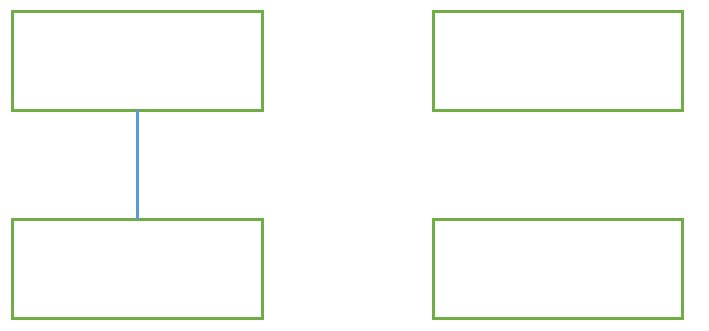
\includegraphics[scale=0.8]{文字文稿1.pdf}}
		\caption{这里是图片的标题}\label{fig:picturename3}
	\end{figure}
	\subsection{模型的评价}
	\begin{itemize}
		\item \textbf{模型的优点}:
			\begin{enumerate}
				\item ……
				\item ……
			\end{enumerate}
		\item \textbf{模型的缺点}:
			\begin{enumerate}
				\item ……
				\item ……
				\item ……
			\end{enumerate}
		\item \textbf{模型的改进}:
			\begin{enumerate}
				\item ……
				\item ……
				\item ……
			\end{enumerate}
	\end{itemize}
	\subsection{模型的推广}

	\newpage
	\phantomsection
	\addcontentsline{toc}{section}{\textbf{参考文献}}
	\begin{thebibliography}{99}
	\bibitem{Paper:刘柳}刘柳. 基于QAR数据的着陆阶段飞行风险研究[D].重庆大学,2018.
	\bibitem{Paper:龙海江}龙海江. 基于QAR数据的重着陆分析研究[D].中国民用航空飞行学院,2020.DOI:10.27722/d.cnki.gzgmh.2020.000089.
	
	\end{thebibliography}

	\newpage

	\phantomsection
	\addcontentsline{toc}{section}{\textbf{附\hspace{2pc}录}}

	% \appendix
	% \ctexset{section={format={\zihao{-4}\heiti\raggedright}}}
	\begin{center}
		\heiti\zihao{4} 附\hspace{2pc}录
	\end{center}

% \phantomsection
% \addcontentsline{toc}{subsection}{[A]图示}
	% \section*{[A]图示}
	\noindent{\heiti [A]图示}

\newpage
% \phantomsection
% \addcontentsline{toc}{subsection}{[B]支撑文件列表}
	% \section*{[B]支撑文件列表}
	\noindent{\heiti [B]支撑文件列表}
	~\\

	支撑文件列表如下(列表中不包含原始数据集):

\newpage
% \phantomsection
% \addcontentsline{toc}{subsection}{[C]使用的软件、环境}
	% \section*{[C]使用的软件、环境}
	\noindent{\heiti [C]使用的软件、环境}
	~\\

	为解决该问题,我们所使用的主要软件有:
	
	Python环境下所用使用到的库及其版本如下:

\newpage
% \phantomsection
% \addcontentsline{toc}{subsection}{[D]问题解决源程序}
	% \section*{[D]问题解决源程序}
\noindent{\heiti [D]问题解决源程序}

% \phantomsection
% \addcontentsline{toc}{subsubsection}{D.1}
\textbf{D.1 }
\begin{python}
import numpy as np
\end{python}
\newpage
% \phantomsection
% \addcontentsline{toc}{subsubsection}{D.2}
\textbf{D.2 }

\newpage
% \phantomsection
% \addcontentsline{toc}{subsubsection}{D.3}
\textbf{D.3 }

\newpage
% \phantomsection
% \addcontentsline{toc}{subsubsection}{D.4}
\textbf{D.4 }

\end{document}